\section{Methods}
\label{sec:methods}
% NOT finished

% \subsection{The Challenge Database}
% \label{subsec:database}
% % finished

% The challenge database \cite{Oliveira_2021_CirCor} provides multiple PCG recordings collected at different auscultation locations for a number of young subjects. The annotations of the existence of heart murmurs are provided for each recording, along with annotations for heart sound segmentation annotation. The clinical outcomes are provided for each subject. For algorithm development, we divided the public subset of the challenge database into the training set and the validation set with a ratio of 8:2. This split was stratified on the categorical attributes ``Age'', ``Sex'', ``Pregnancy status'' and the prediction targets ``Murmur'', ``Outcome''.


\subsection{Preprocess Pipeline}
\label{subsec:preproc}
% finished

After a careful study of spectral characteristics of heart murmurs from medical literature \cite{Donnerstein_1989, Noponen_2007}, and with reference to previous work \cite{Schmidt_2010}, we constructed the PCG signal preprocessing pipeline as follows:
\begin{itemize}
    \item Resample to 1000 Hz;
    \item Butterworth bandpass filtering of order 3 and cutoff frequencies 25 - 400 Hz;
    \item Z-score normalization to zero mean and unit variance.
\end{itemize}

\subsection{Neural Network Backbones}
\label{subsec:backbone}
% almost finished

Inspired by the work of \texttt{wav2vec2} \cite{baevski2020wav2vec}, and under the consideration of exploring and utilizing the powerfulness of pretraining models on larger databases \cite{wolf-etal-2020-transformers}, we adopted a shrunken \texttt{wav2vec2} as one of our neural network backbones. We used the time-domain signals, namely the PCG waveforms, as model input, rather than the derived time-frequency-domain signals, for example, the spectrogram. Since PCG signals have significantly lower sampling frequencies than conventional human voice audio signals, we reduced the dimension (number of channels) of the `wav2vec2` model's encoder and its depth (number of hidden layers).

% The `wav2vec2` model has a small block of convolutions in the bottom used as the feature extractor which extracts feature maps of a fixed dimension from the waveforms and feeds into ...


% \begin{table}[!htp]
% \centering
% \begin{tabular}{r|l}
%     \hline
%     Backbone & \# Params \\ \hline
%     MultiBranch \cite{Kang_2022_cinc2021_iop} & 17.7M \\
%     SE-ResNet \cite{Kang_2022_cinc2021_iop} & 15.9M \\
%     ResNet-NC \cite{ribeiro2020automatic} & 15.4M \\
%     TResNetS \cite{Kang_2022_cinc2021_iop} & 41.0M \\
%     TResNetF \cite{Kang_2022_cinc2021_iop} & 4.0M \\
%     wav2vec2 \cite{baevski2020wav2vec} & 19.8M \\ \hline
% \end{tabular}
% \caption{to write.}
% \label{tab:nn_backbone}
% \end{table}

\begin{table}[!htp]
\centering
\begin{tabular}{r|l}
    \hline
    Backbone & \# Params \\ \hline
    MultiBranch & 17.7M \\
    SE-ResNet & 15.9M \\
    ResNet-NC & 15.4M \\
    TResNetS & 41.0M \\
    TResNetF & 4.0M \\
    wav2vec2 & 19.8M \\ \hline
\end{tabular}
\caption{to write.}
\label{tab:nn_backbone}
\end{table}


Considering that PCG signals share a similar physiological origin as electrocardiogram (ECG) signals, we further adjusted and tested several neural network backbones that have proven effective in ECG problems, including multi-branch convolutional neural networks (MultiBranch), SE-ResNet, TResNetS, TResNetF \cite{Kang_2022_cinc2021_iop}, and ResNet-NC \cite{ribeiro2020automatic} etc. We enlarged the kernel sizes of each convolution in these backbones by a factor of 2, which is the ratio of the sampling frequencies.

The efficacy of the neural network backbones is validated via experiments as illustrated in Figure \ref{fig:compare_nn}.


\begin{figure}[!htp]
\centering
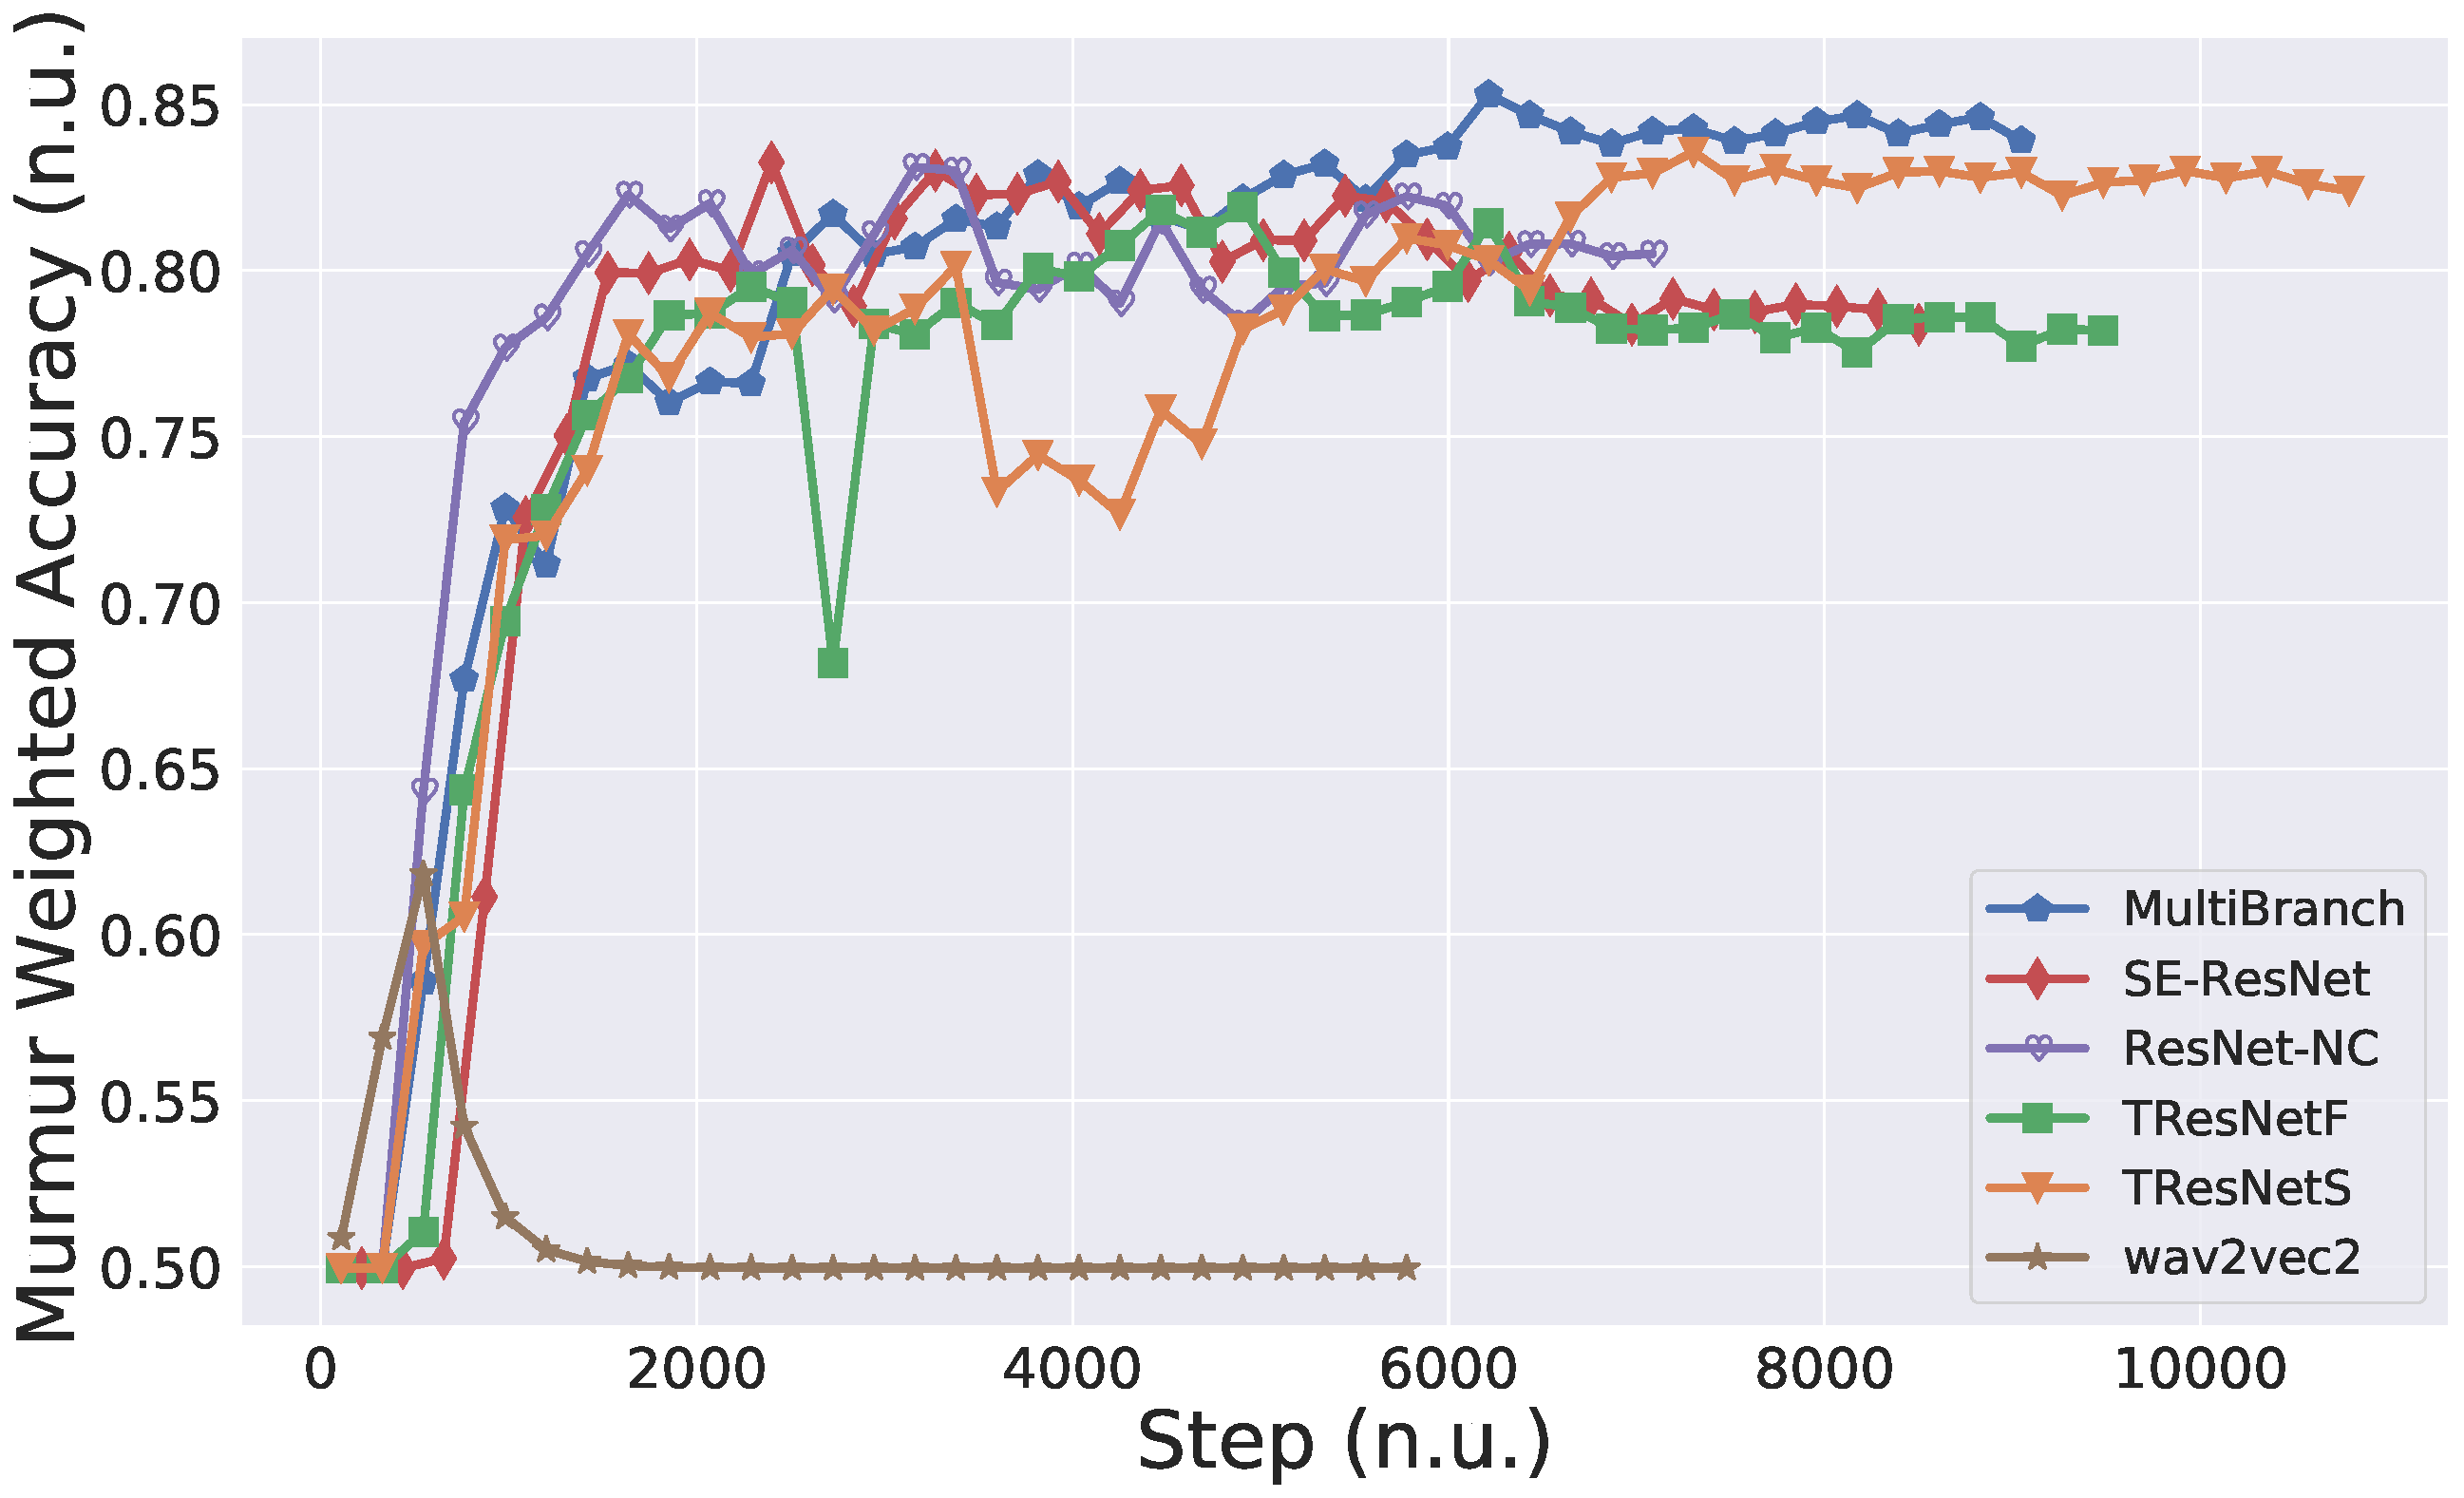
\includegraphics[width=\linewidth]{images/compare_nn.pdf}
\caption{Curve of weighted accuracies of murmur detection on the validation set \ref{subsec:training} using 7 different neural network backbones. The model heads, optimizers, loss functions, as well as other training setups, were kept the same.}
\label{fig:compare_nn}
\end{figure}


\subsection{Multi-Task Learning}
\label{subsec:mtl}
% NOT finished

The challenge \cite{cinc2022} has 2 per-patient classification tasks:
\begin{itemize}
    \item the prediction of the existence of heart murmurs into 3 classes: ``Present'', ``Unknown'', ``Absent'';
    \item the prediction of clinical outcome of the subject into 2 classes: ``Abnormal'', ``Normal''.
\end{itemize}

It should be noted that the challenge database \cite{Oliveira_2021_CirCor} provides per-recording annotations for the former task and heart sound segmentation annotations as well. We applied the multi-task learning (MTL) paradigm \cite{Caruana_1997_mtl} via hard parameter sharing. More precisely, we use one neural network model for all the tasks. Each task has its specific model head, typically a stack of linear layers concatenated to the shared backbone as discussed in Section \ref{subsec:backbone}.

TODO: add a figure of the MTL paradigm


\begin{figure*}
\centering
\begin{subfigure}[b]{0.49\linewidth}
    \centering
    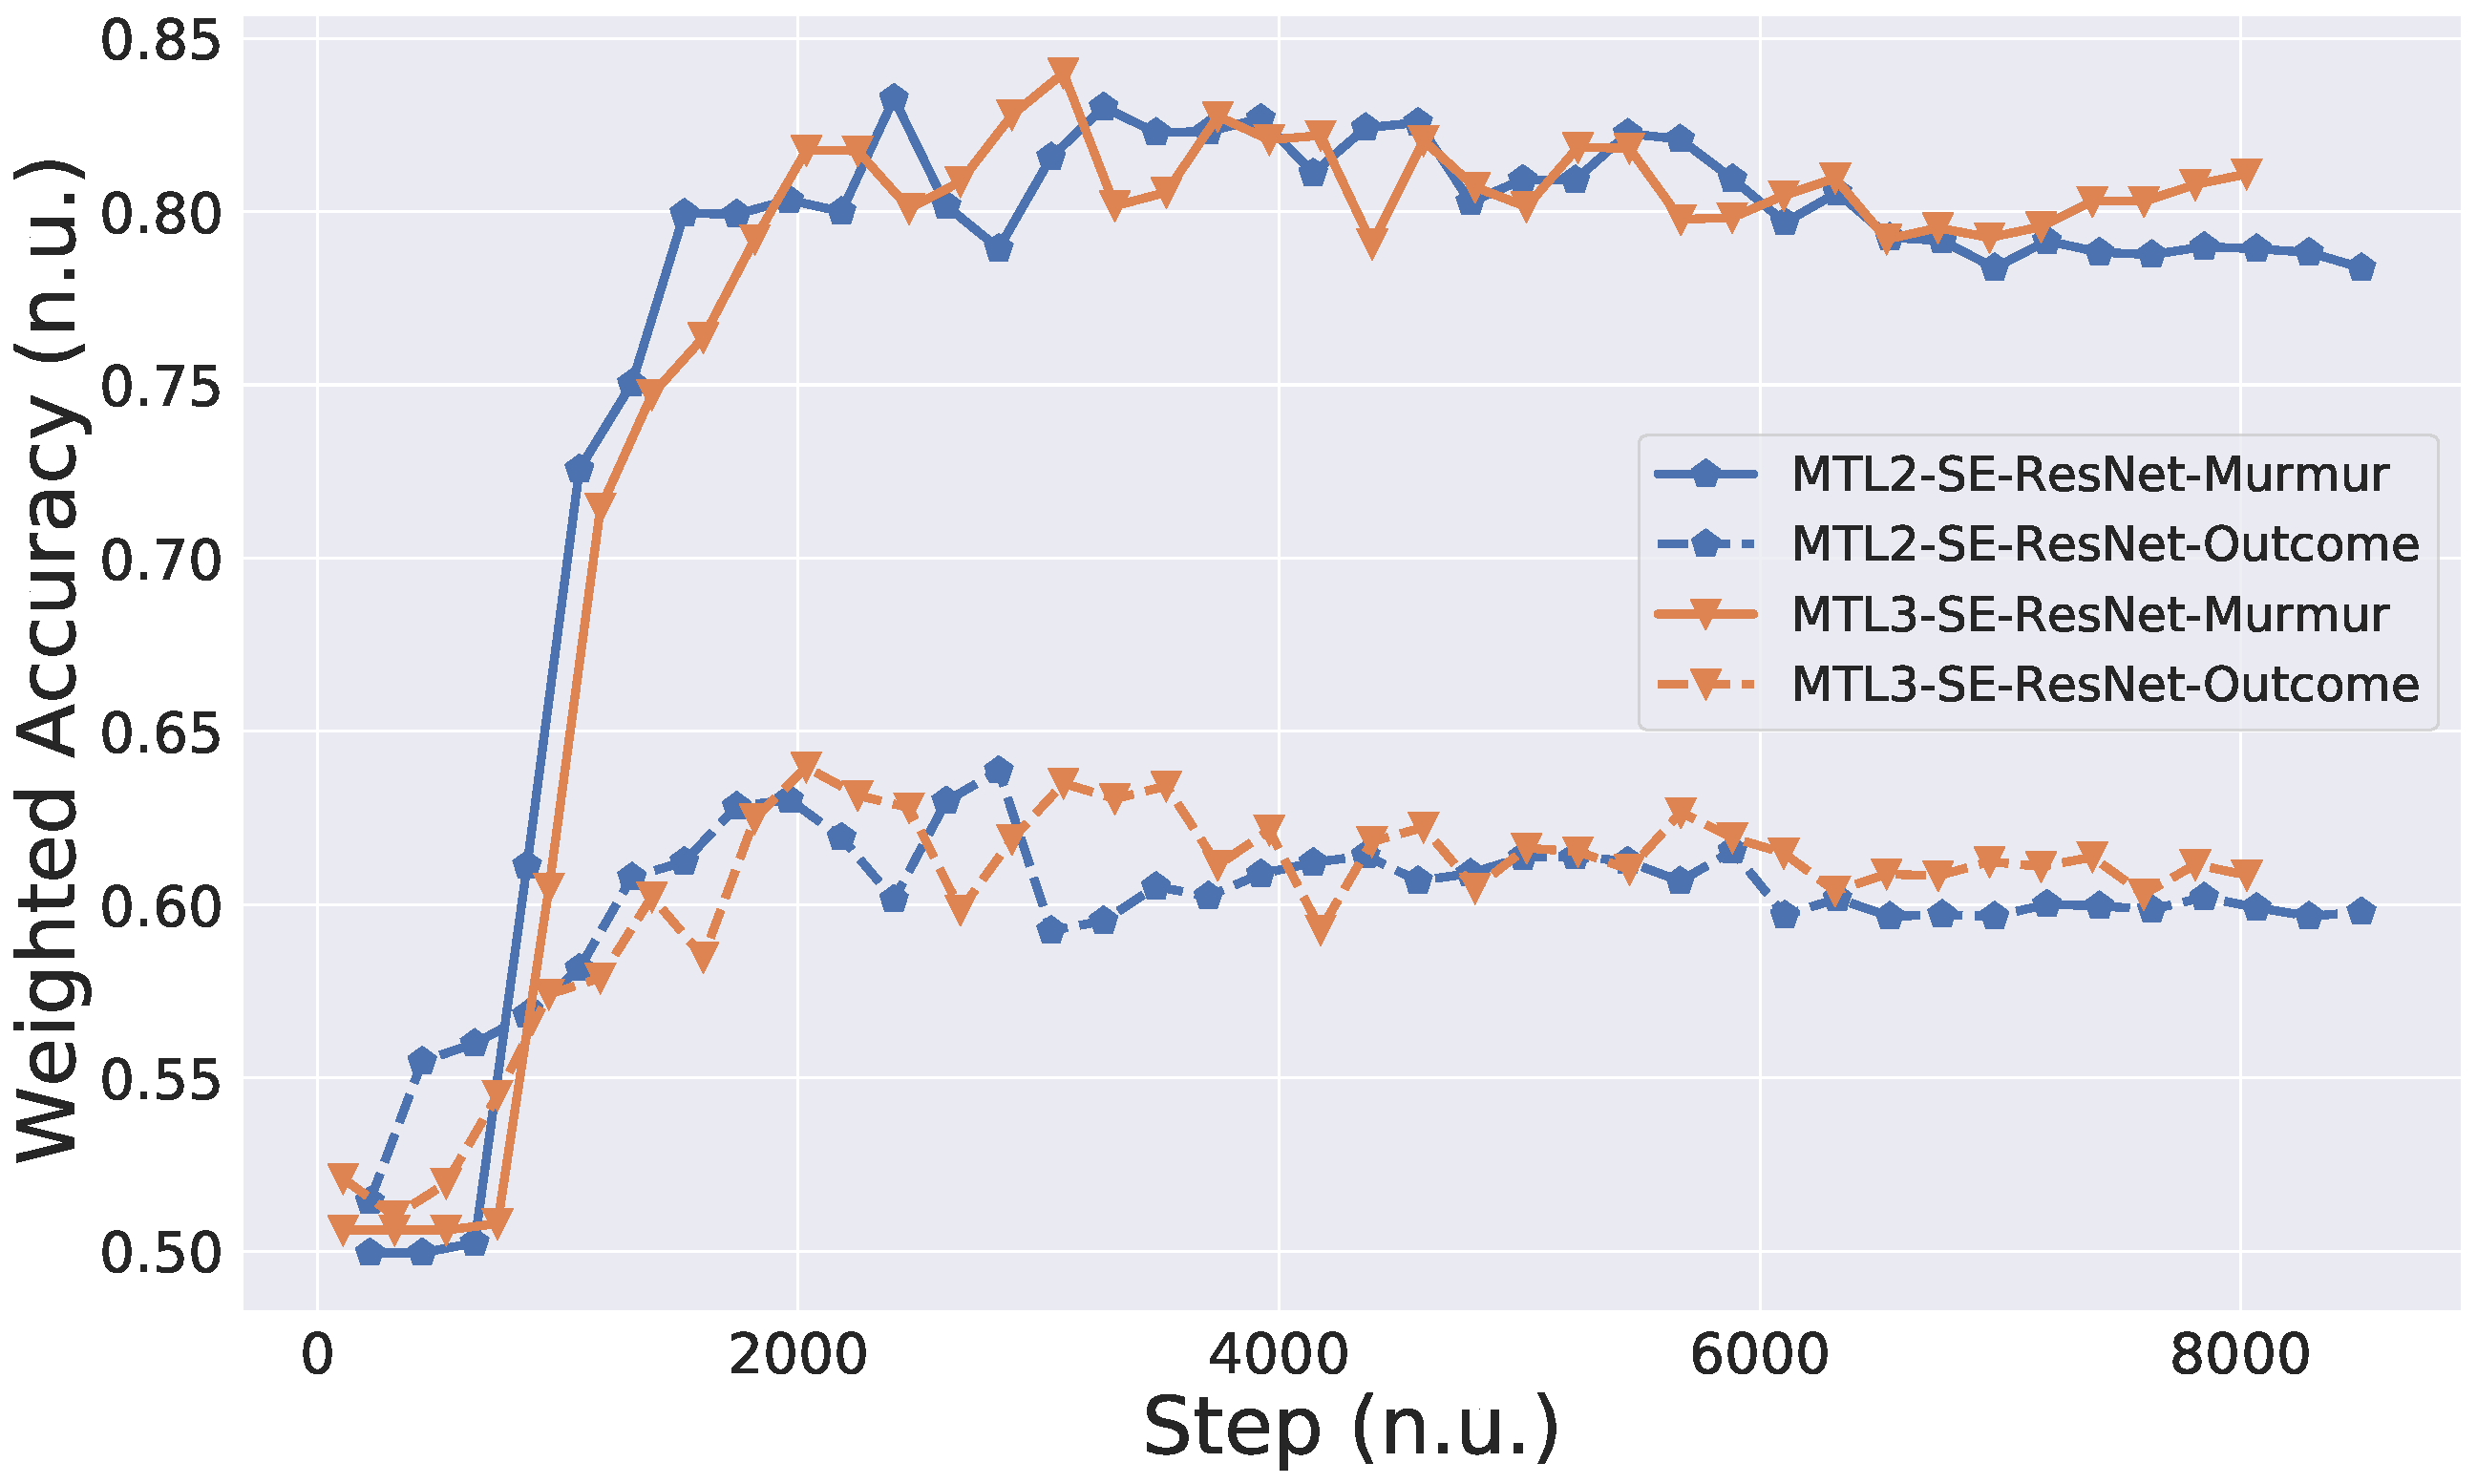
\includegraphics[width=\textwidth]{images/se-resnet-clf-vs-mtl.pdf}
    \caption[]
    {to write.}
    \label{fig:se-resnet-clf-vs-mtl}
\end{subfigure}
\hfill
\begin{subfigure}[b]{0.49\linewidth}
    \centering
    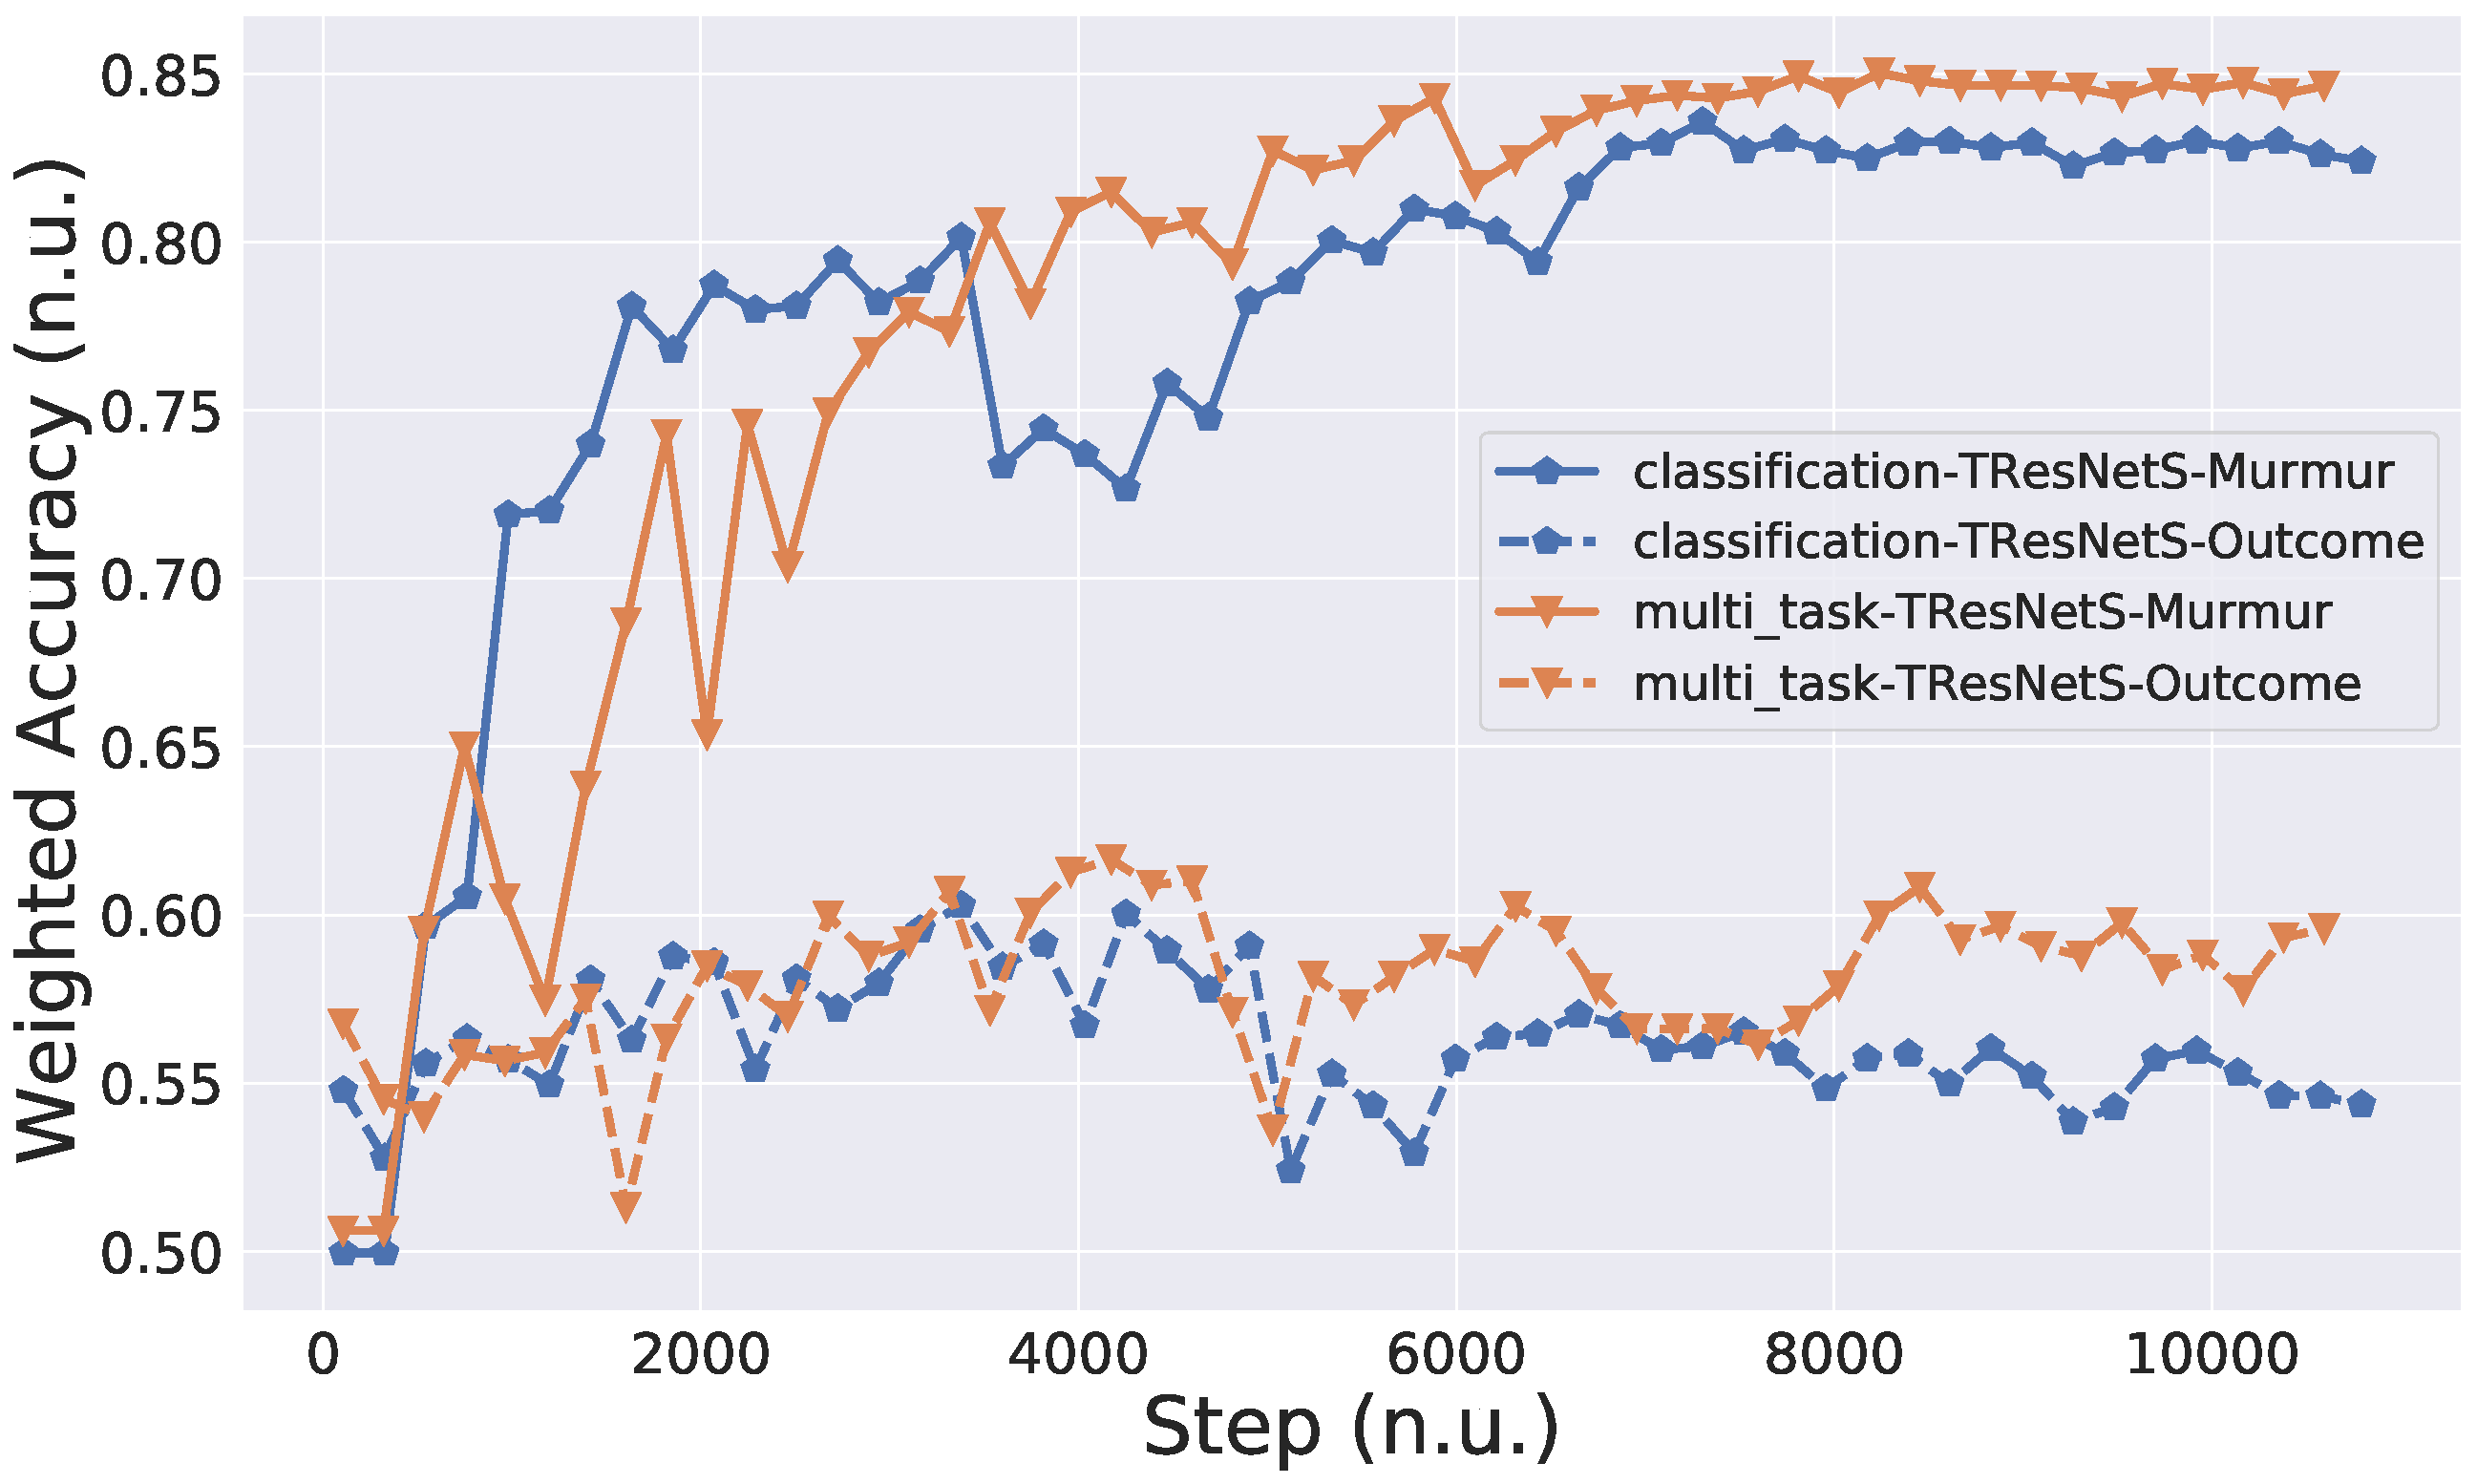
\includegraphics[width=\textwidth]{images/tresnets-clf-vs-mtl.pdf}
    \caption[]
    {to write}
    \label{fig:tresnets-clf-vs-mtl}
\end{subfigure}
\caption[]
{to write.}
\label{fig:mtl}
\end{figure*}


As depicted in Figure \ref{fig:mtl}, experiments showed that models (with the same backbone) using an additional segmentation head (denoted as ``MTL3'') usually outperformed models with only two classification heads (denoted as ``MTL2'') for the challenge tasks.

\subsection{Training Setups}
\label{subsec:training}
% NOT finished

For algorithm development, we divided the publicly available part of the challenge database into the training set and the validation set with a ratio of 8:2. This split was stratified on the categorical attributes ``Age'', ``Sex'', ``Pregnancy status'' and the prediction targets ``Murmur'', ``Outcome''.

TODO: write more....

To alleviate overfitting on the training set and to improve model transferability, during the neural network training process, we applied several types of augmentations to the batched training data stochastically:
\begin{itemize}
    \item to write
    \item to write
\end{itemize}

TODO: loss, optimizers, etc.

% 
% \begin{figure*}
% \centering
% \begin{subfigure}[b]{0.49\linewidth}
%     \centering
%     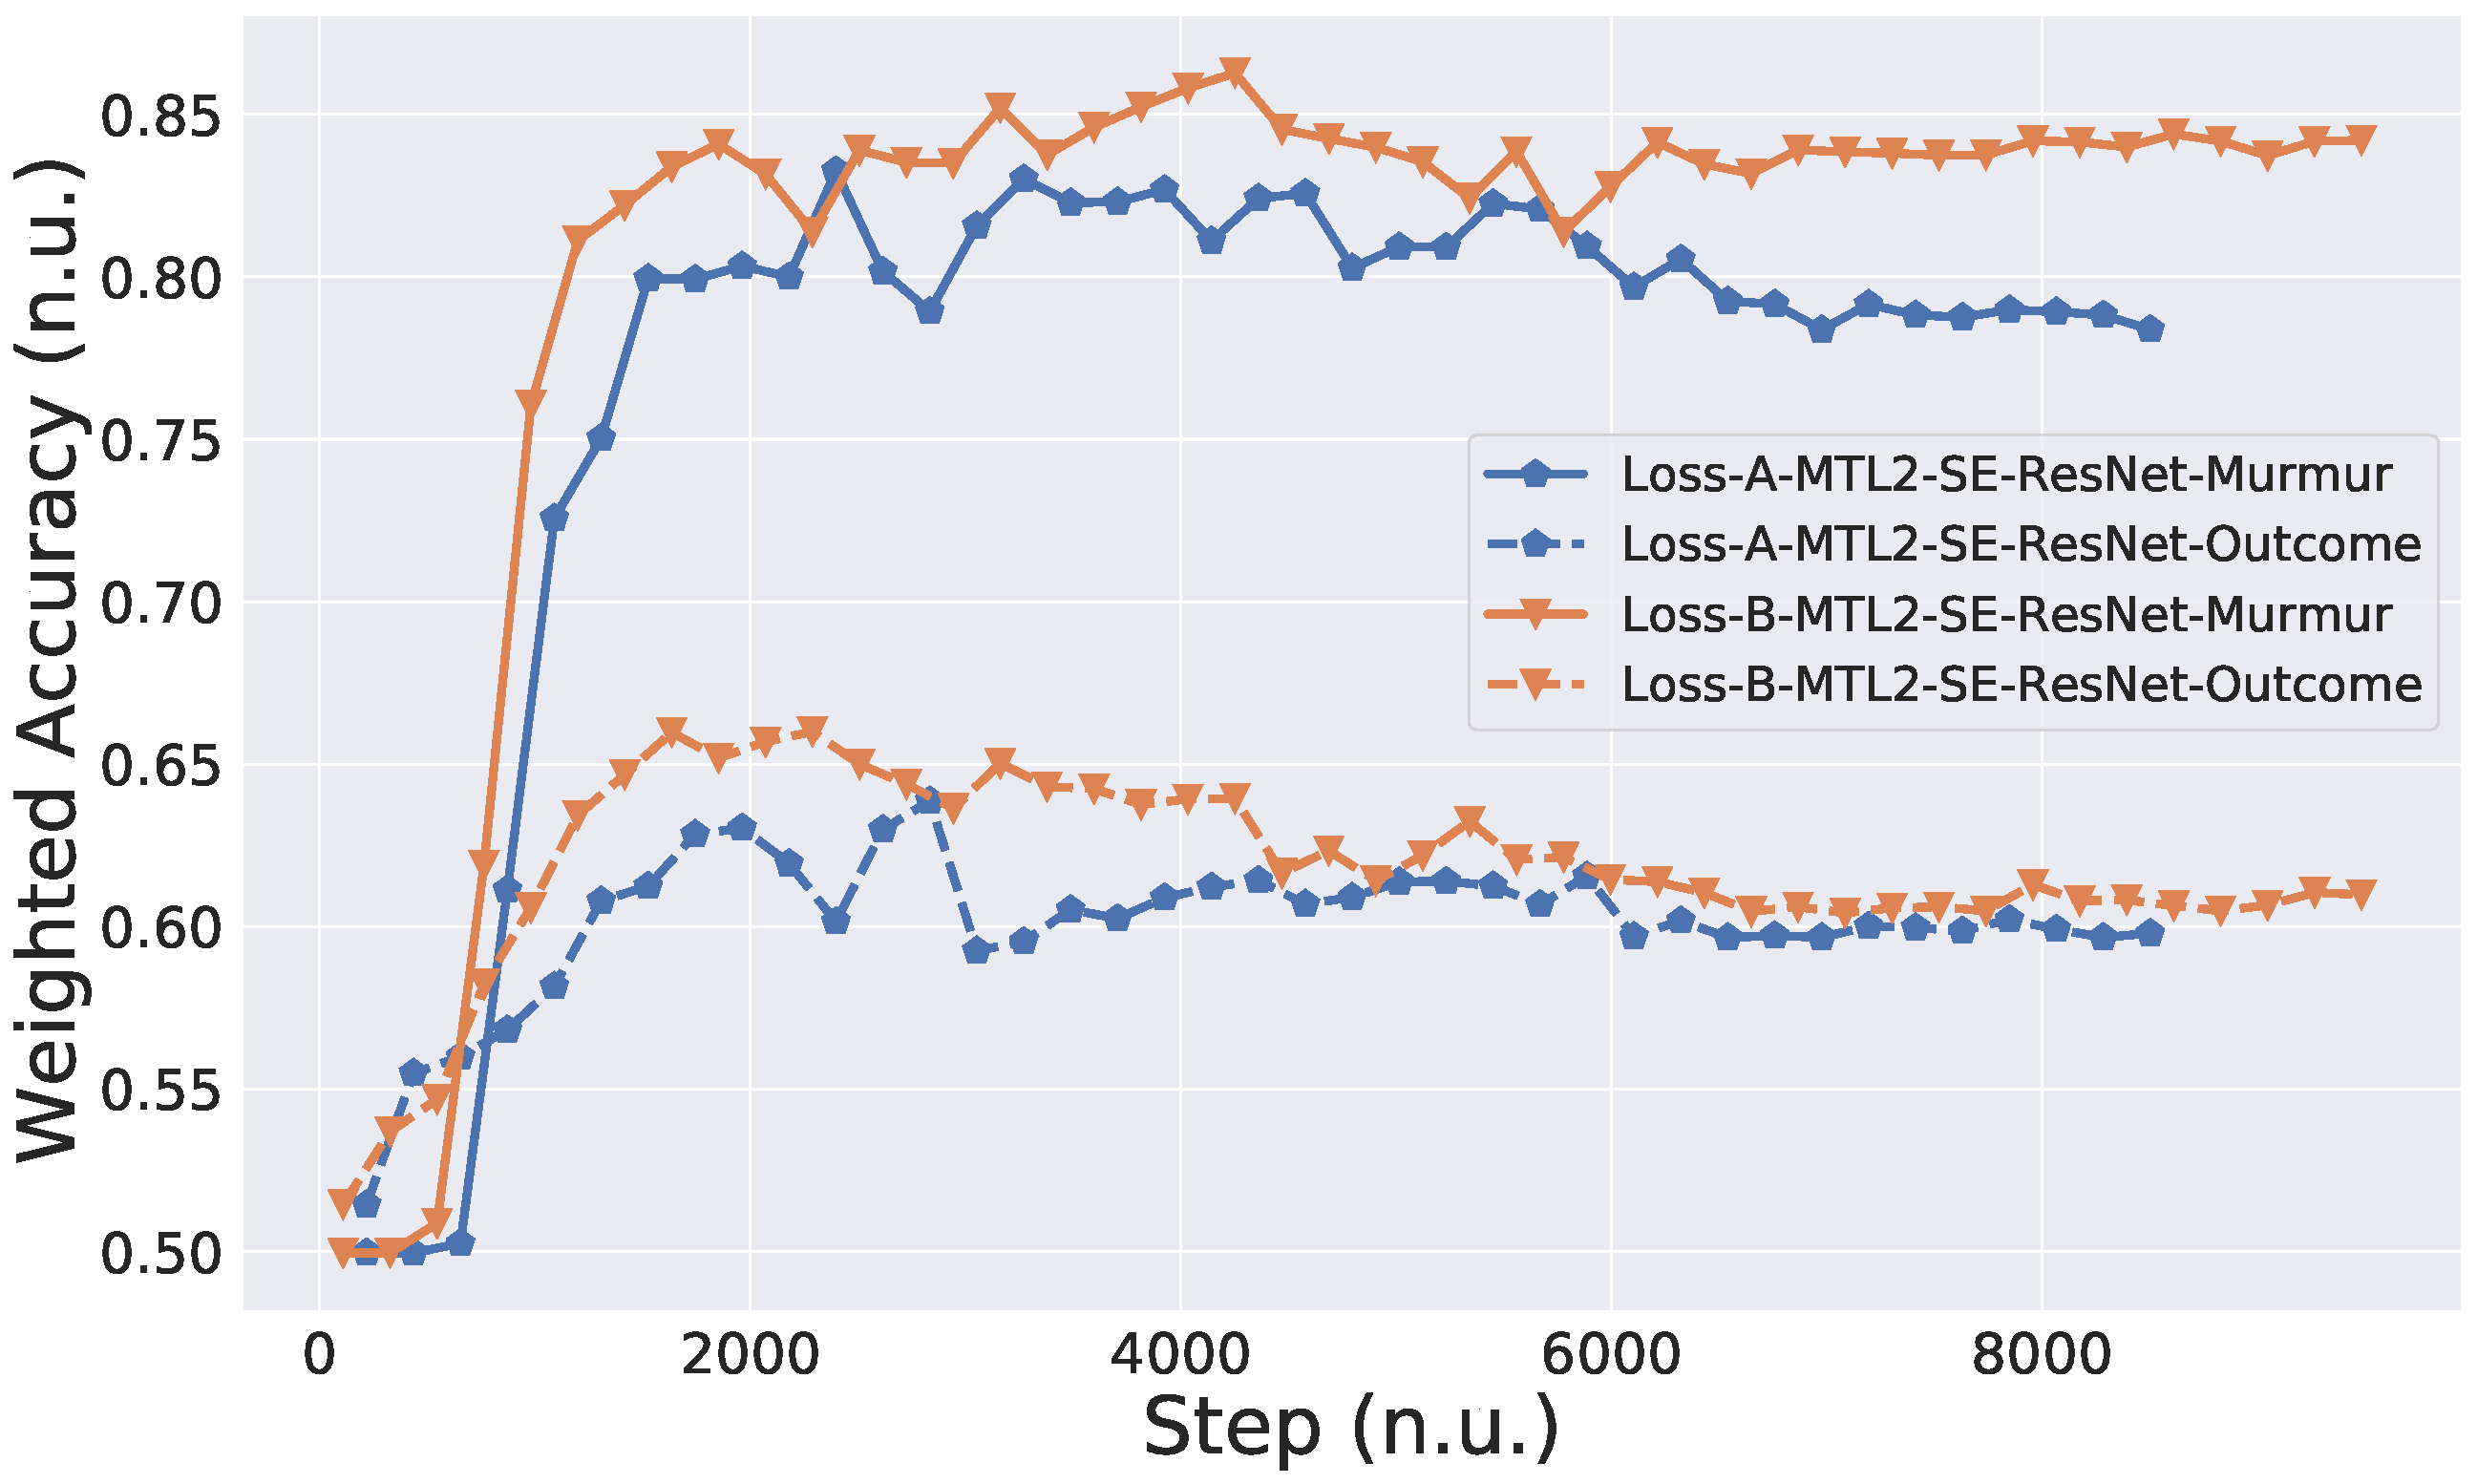
\includegraphics[width=\textwidth]{images/clf-se-resnet-lossA-vs-lossB.pdf}
%     \caption[]
%     {to write.}
%     \label{fig:clf-se-resnet-lossA-vs-lossB}
% \end{subfigure}
% \hfill
% \begin{subfigure}[b]{0.49\linewidth}
%     \centering
%     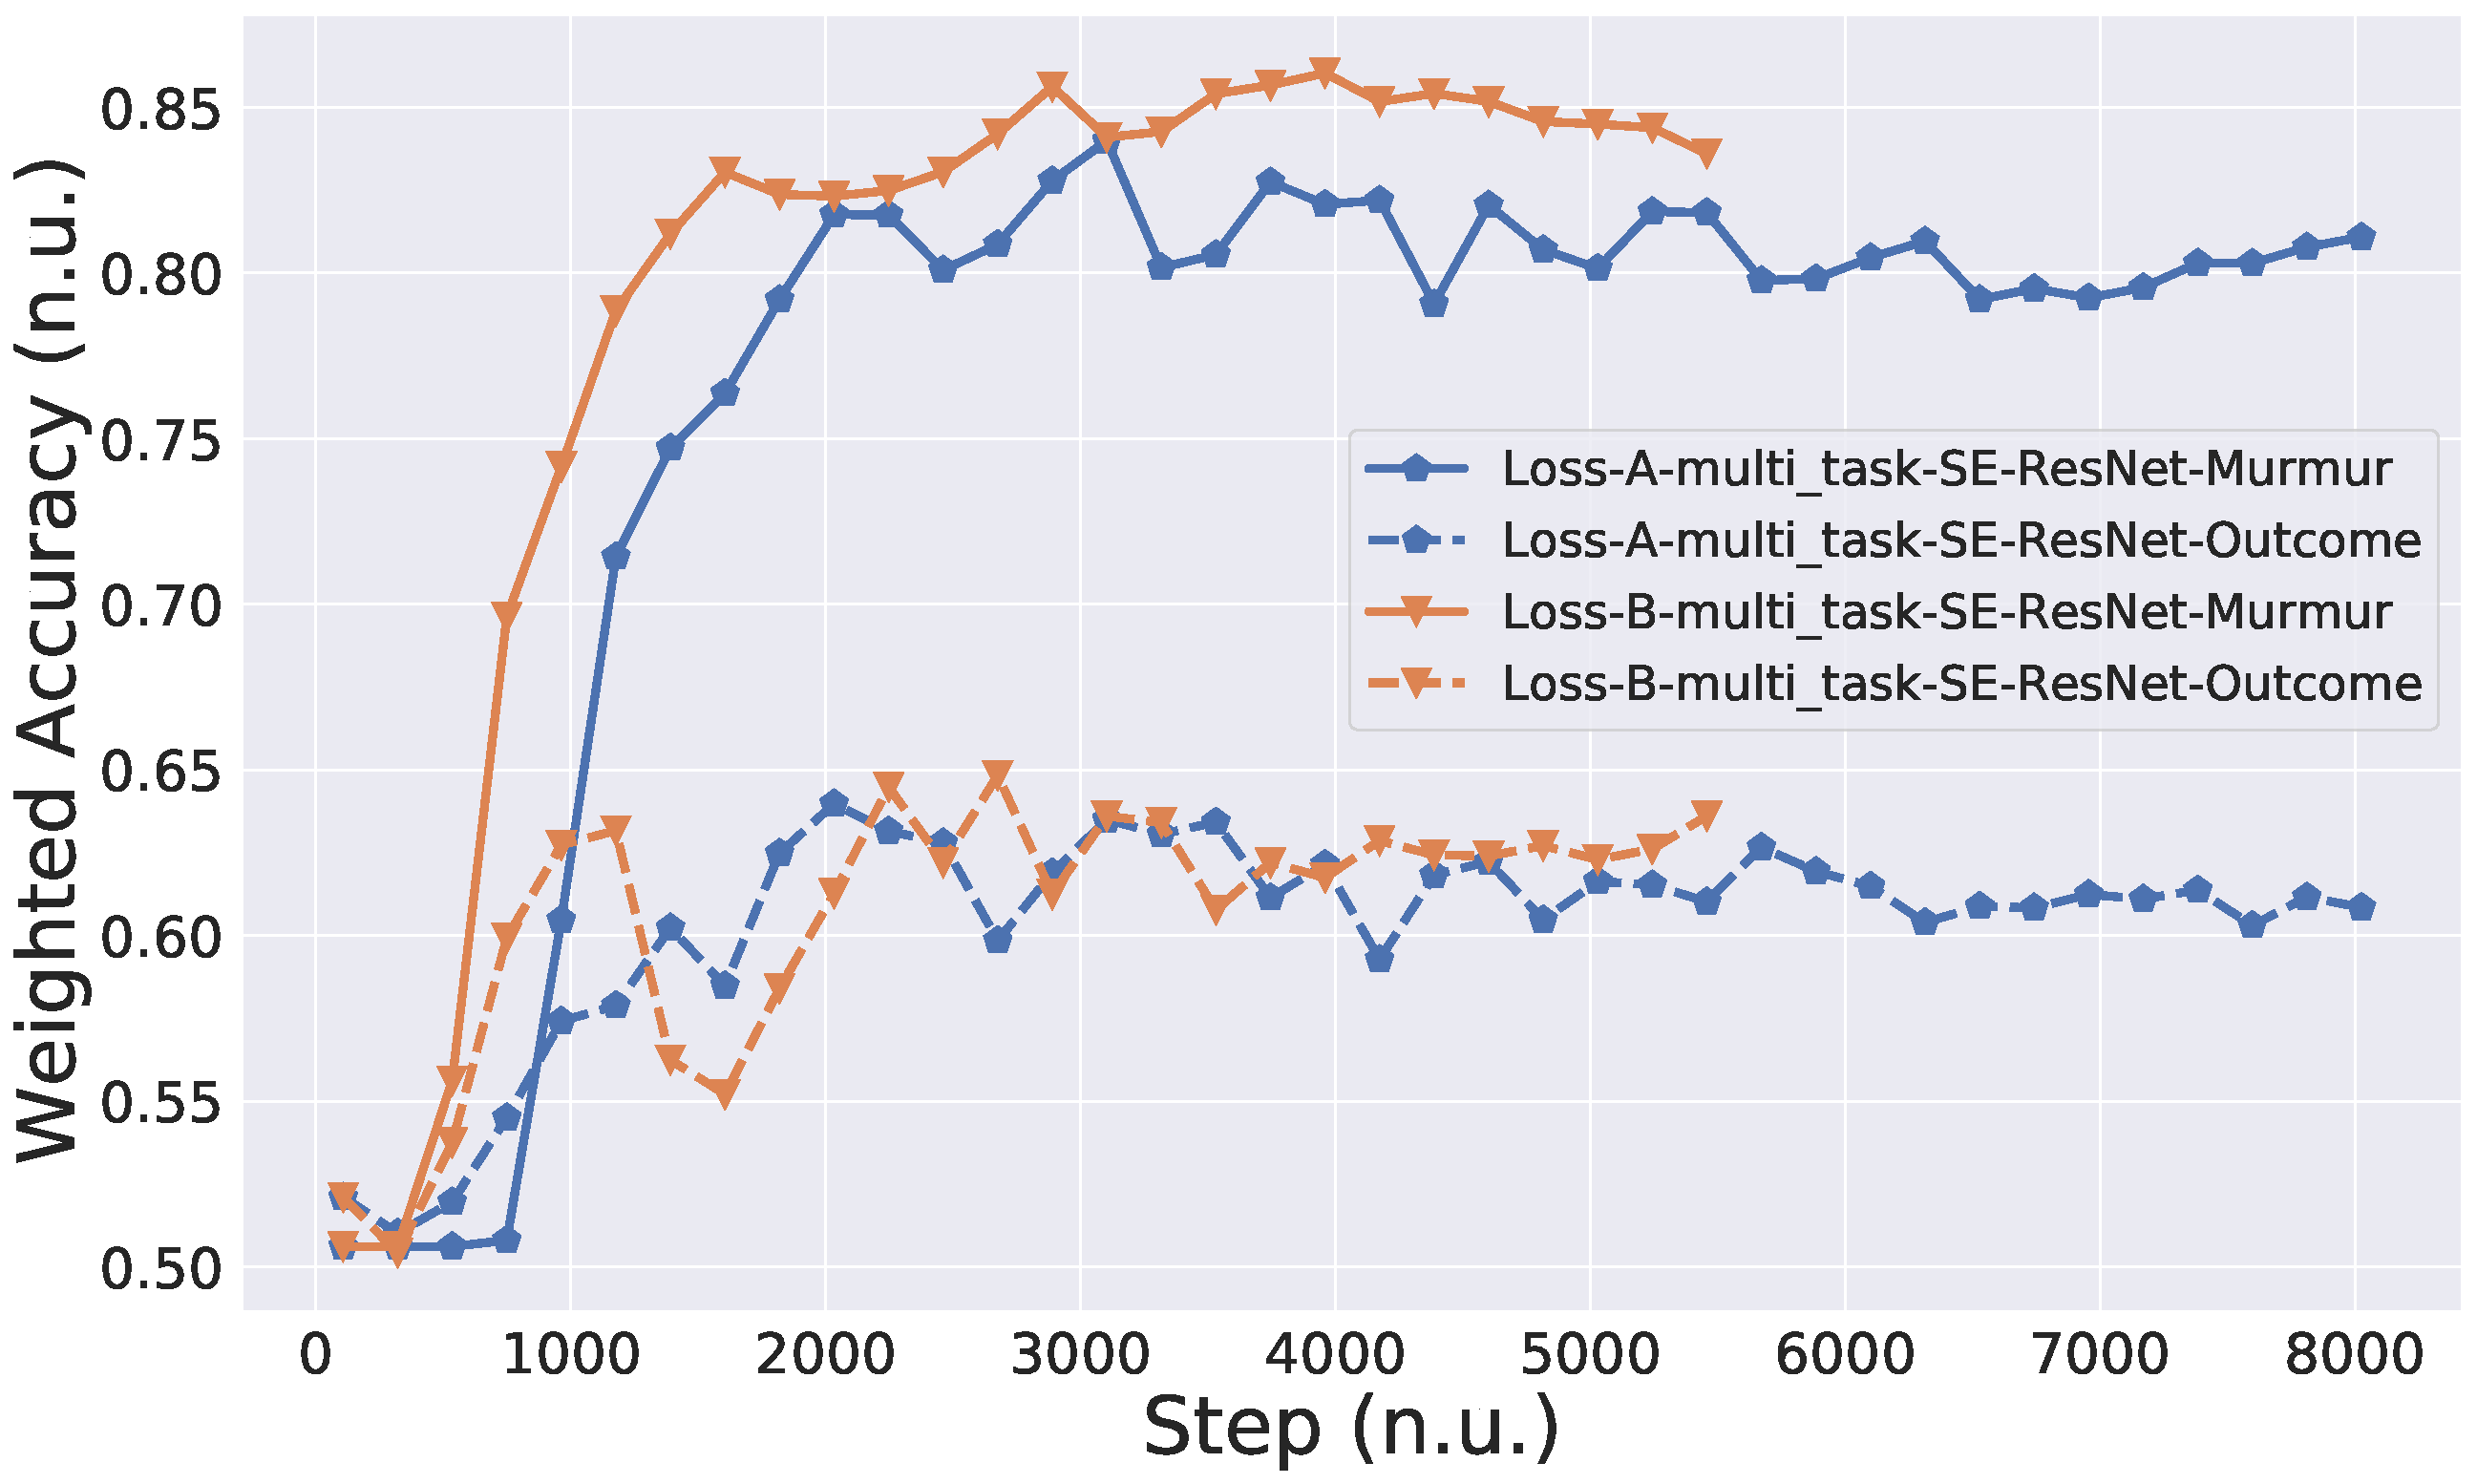
\includegraphics[width=\textwidth]{images/mtl-se-resnet-lossA-vs-lossB.pdf}
%     \caption[]
%     {to write}
%     \label{fig:mtl-se-resnet-lossA-vs-lossB.pdf}
% \end{subfigure}
% \caption[]
% {to write.}
% \label{fig:loss}
% \end{figure*}

\begin{figure}[!htp]
\centering
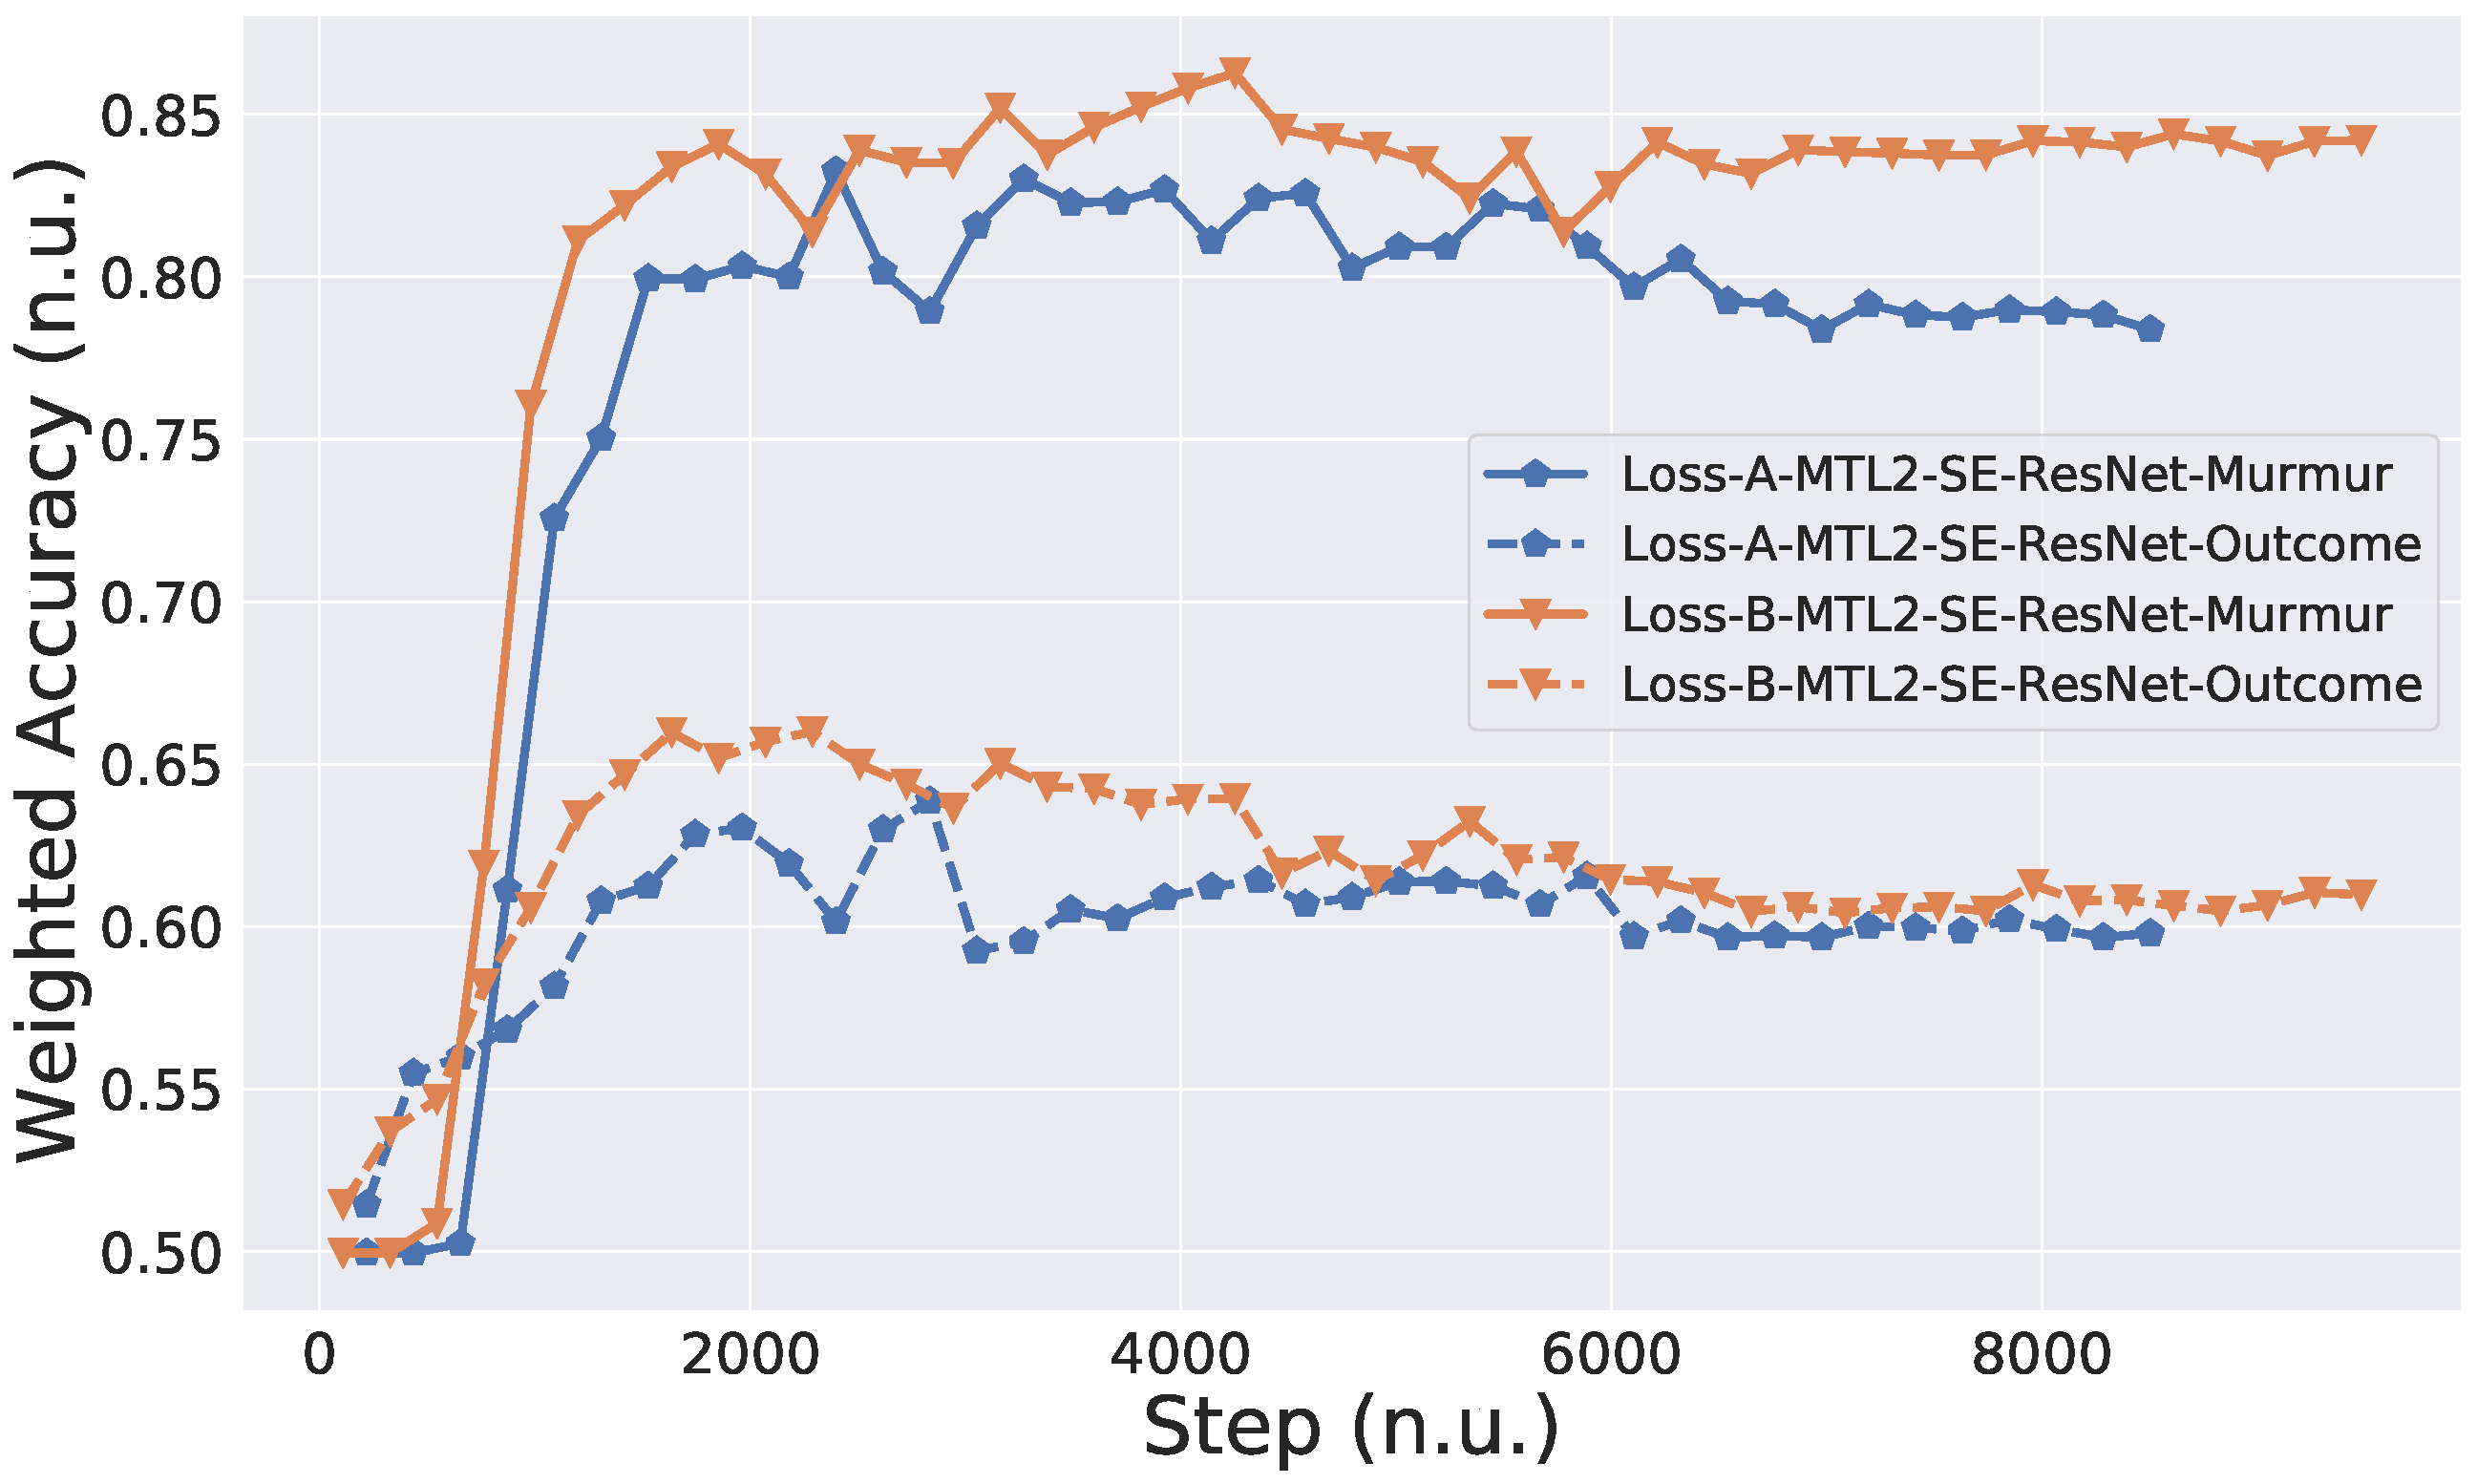
\includegraphics[width=\linewidth]{images/clf-se-resnet-lossA-vs-lossB.pdf}
\caption[]
{Experiments to compare the 2 loss functions. The model with 2 classification heads and with SE-ResNet as the backbone was used.}
\label{fig:clf-se-resnet-lossA-vs-lossB}
\end{figure}


\subsection{Demographic Features}
\label{subsec:demo_feat}
% NOT finished

\begin{figure}[!htp]
\centering
\begin{subfigure}[b]{0.49\linewidth}
    \centering
    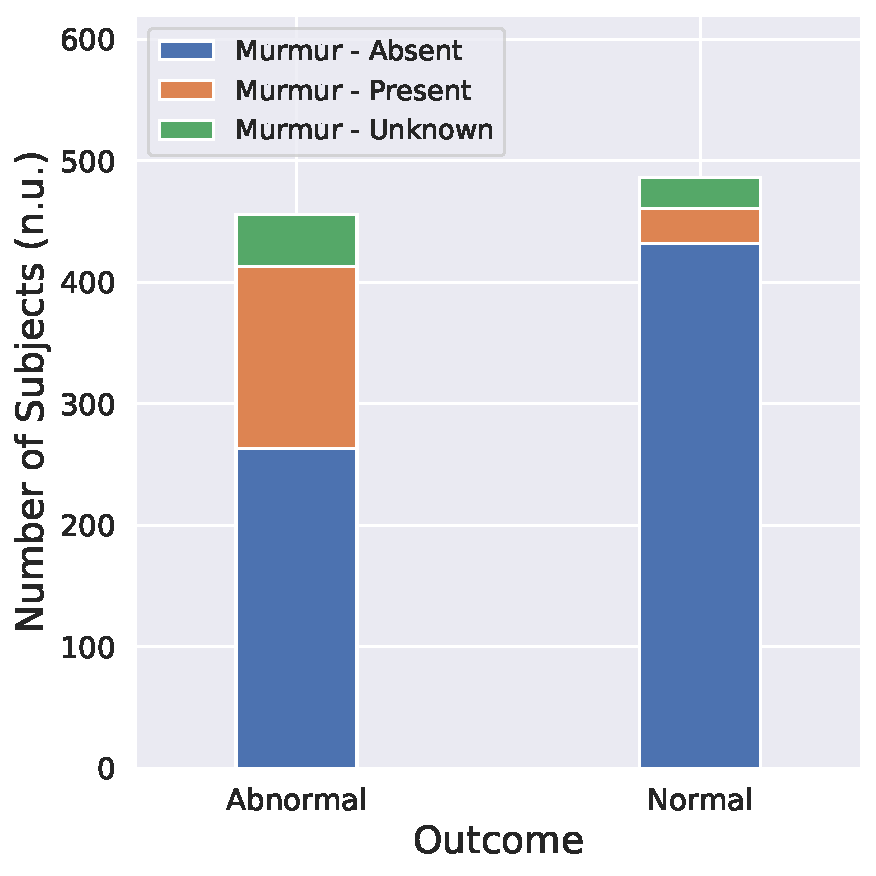
\includegraphics[width=\textwidth]{images/outcome_murmur_corr.pdf}
    \caption[]
    {Distribution of outcome against the existence of heart murmurs.}
    \label{fig:outcome_murmur_corr}
\end{subfigure}
\hfill
\begin{subfigure}[b]{0.49\linewidth}
    \centering
    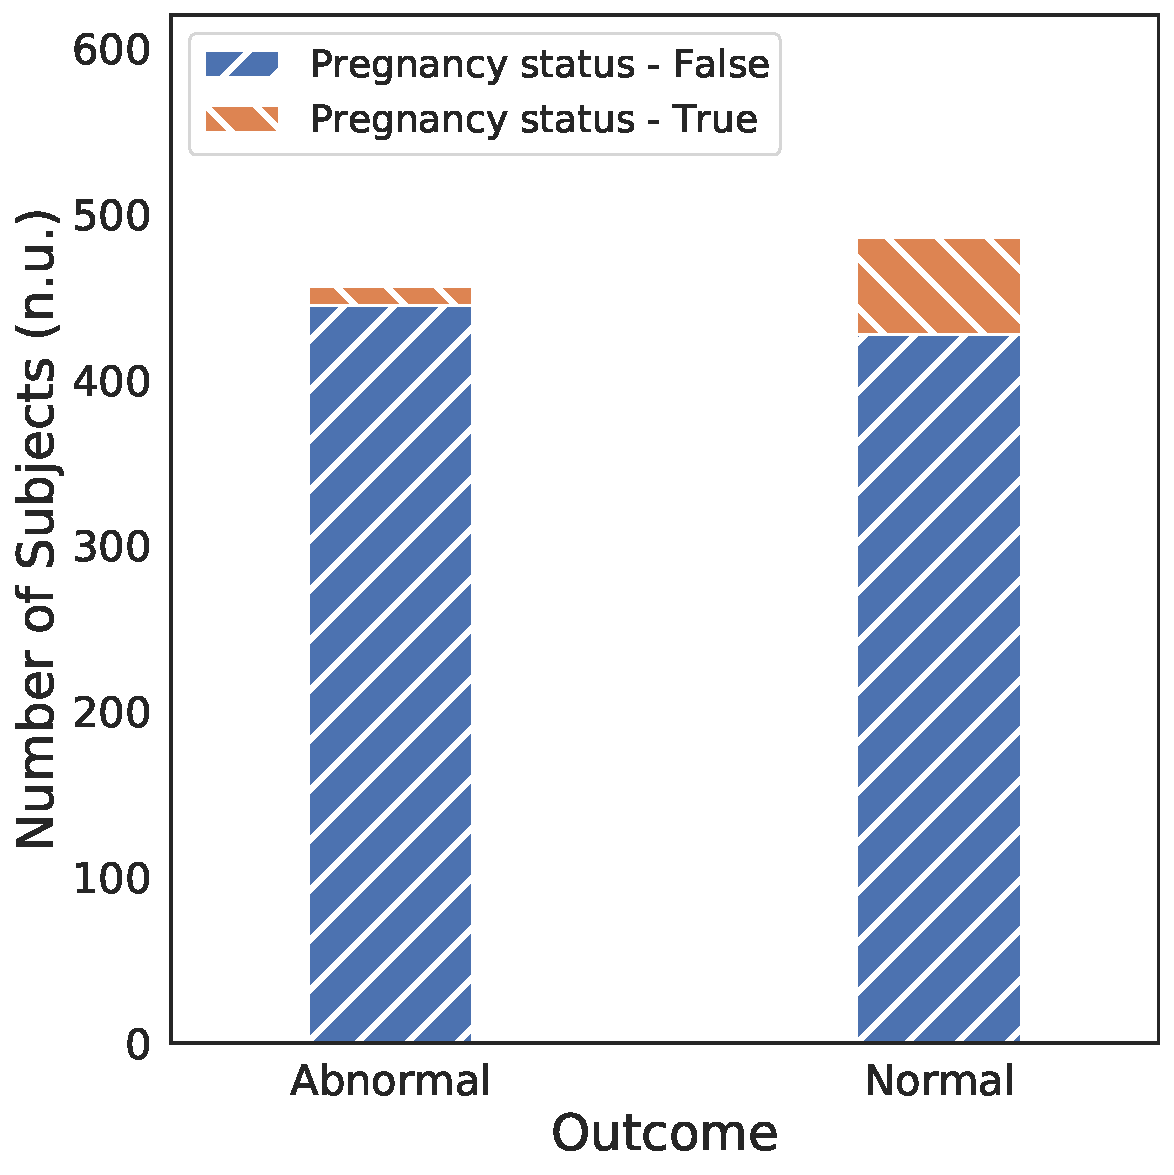
\includegraphics[width=\textwidth]{images/outcome_pregnancy_status_corr.pdf}
    \caption[]
    {Distribution of outcome against pregnancy status.}
    \label{fig:outcome_pregnancy_status_corr}
\end{subfigure}
\vskip\baselineskip
\begin{subfigure}[b]{0.49\linewidth}
    \centering
    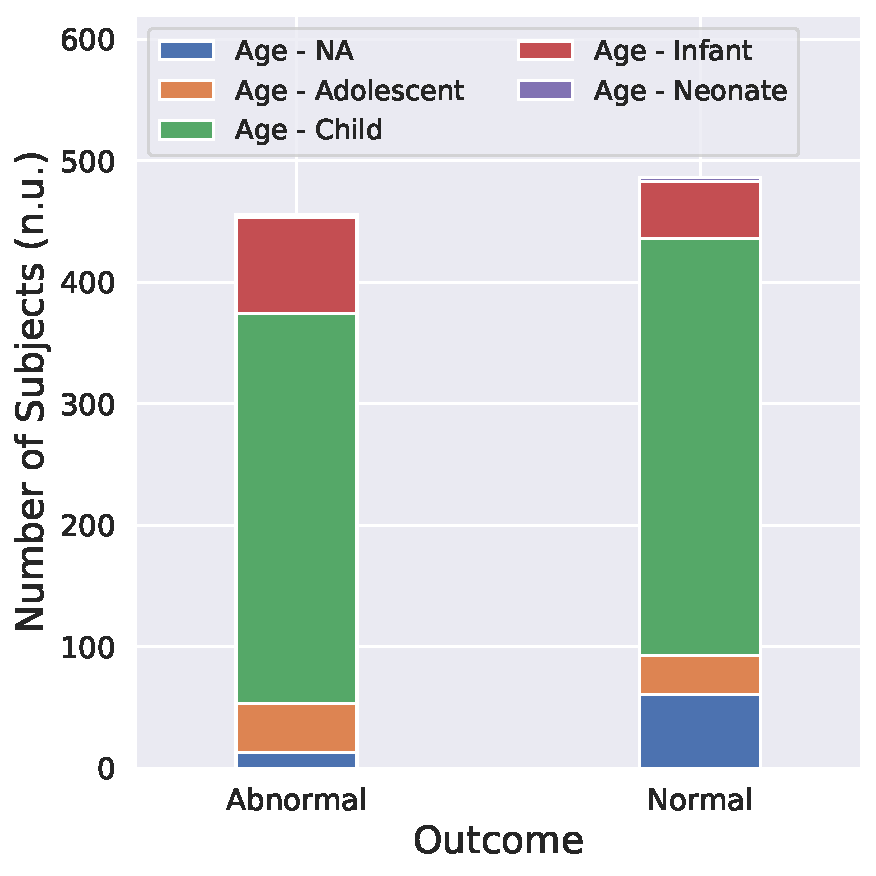
\includegraphics[width=\textwidth]{images/outcome_age_corr.pdf}
    \caption[]
    {Distribution of outcome against age.}
    \label{fig:outcome_age_corr}
\end{subfigure}
\hfill
\begin{subfigure}[b]{0.49\linewidth}
    \centering
    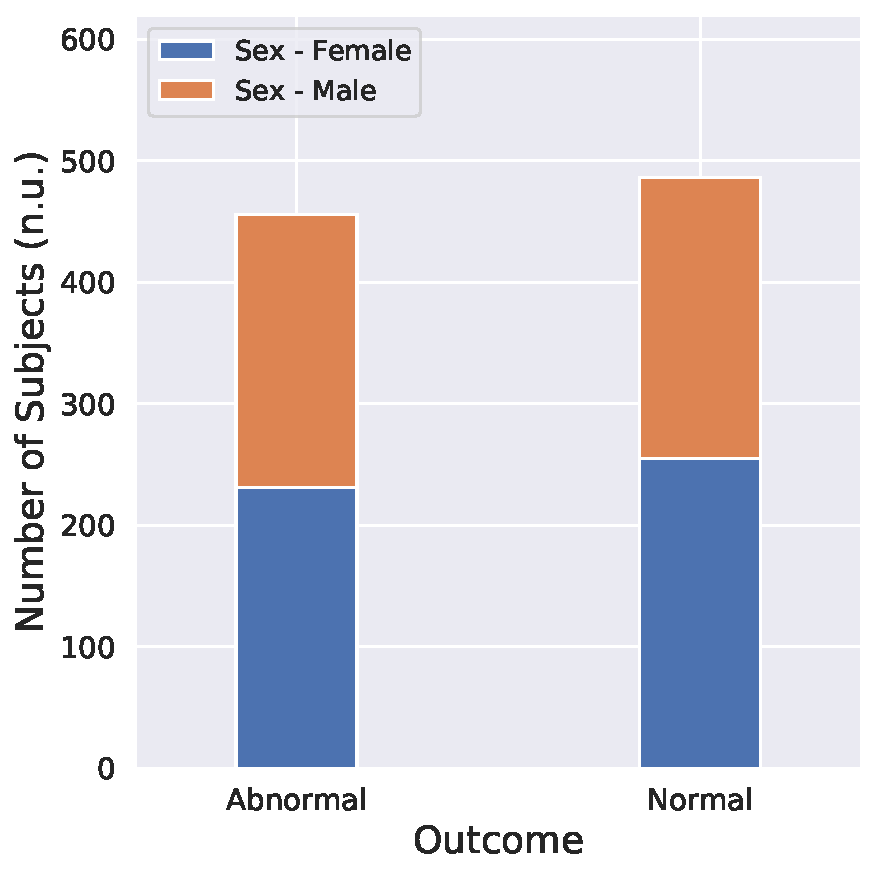
\includegraphics[width=\textwidth]{images/outcome_sex_corr.pdf}
    \caption[]
    {Distribution of outcome against sex.}
    \label{fig:outcome_sex_corr}
\end{subfigure}
\caption[]
{Distribution of outcome against 4 typical categorical demographic variables.}
\label{fig:outcome_corr}
\end{figure}
